\documentclass[UTF8,a4paper,12pt]{ctexart}
\usepackage{geometry}
\usepackage{amsmath}
\usepackage{graphicx}
\usepackage{booktabs}
\usepackage{float}
\usepackage{hyperref}
\usepackage{setspace}
\usepackage{caption}
\geometry{left=2.5cm,right=2.5cm,top=2.5cm,bottom=2.5cm}
\onehalfspacing
\hypersetup{colorlinks=true,linkcolor=black,urlcolor=blue,citecolor=black}
\title{数字政务平台中的公共服务响应效率与风险预警研究}
\author{}
\date{}

\begin{document}
\maketitle

\begin{abstract}
数字政务平台让居民更容易报告日常问题，但“能提交诉求”并不等于“能被及时回应”。本文以纽约 311 为案例，研究公共服务响应是否公平、慢响应与哪些社区机制相关，以及预测结果如何转化为治理行动。本文使用 2023 年纽约 311 数据集，并合并 ACS、HPD数据。结果显示投诉类型的影响最大。Logistic模型在严格时间外推测试中的 AUC 为 0.796；加入目标编码后提升至 0.835，月份分层验证中进一步达到 0.919。ZIP 层面慢响应率与收入中位数显著负相关，与贫困率、住房违规和工作量正相关。时间序列实验显示可通过 4 周移动平均较好预测短期响应压力，优化建模则表明政府在调度时采用风险优先策略能节约最多等待时间，而加入脆弱社区约束可提高公平覆盖。本文认为，311 数据不仅能描述城市问题分布，也能用于诊断公共服务响应差异，并为数字政务平台从被动受理转向主动调度提供依据。本文代码和数据集链接。

\textbf{关键词：}公共服务；响应时间；空间不平等；预测模型；风险预警；调度优化
\end{abstract}

\section{引言}

数字政务平台给了居民提交诉求的平台，但常常不知道需要多久才能得到回应。政府若不能对响应时间作出有效评估也会导致效率低下。

Wang et al. (2016) 的研究反映了城市空间和公共服务需求的差异。Kontokosta, Hong and Korsberg (2017) 则进一步指出，投诉量不仅取决于真实问题多少，也受到居民数字接入能力、维权意识、社会经济条件和对政府信任程度的影响。然而缺少了对“投诉进入系统之后政府如何回应”的关注。即使两个社区都成功提交了投诉，它们是否会被同样及时地处理？慢响应究竟来自哪里？是否可以建立风险预警机制并据此优化调度？


\section{数据与变量}
本文使用纽约市开放数据平台的 \textit{311 Service Requests from 2020 to Present} 数据集。311 是成熟且数据公开程度较高的数字政务平台，可以很好的代表同样存在于其他城市的 12345 热线、政务 App 和城市工单系统等。
样本限定为 2023 年创建且已关闭的请求，并选取六类与日常生活密切相关的投诉：Noise - Residential、HEAT/HOT WATER、UNSANITARY CONDITION、Street Condition、Street Light Condition 和 Traffic Signal Condition。数据清洗包括删除未关闭请求、关闭时间早于创建时间的异常记录、响应时长超过 60 天的极端值，以及行政区或社区板缺失和异常记录。最终样本包含 291645 条投诉。

核心变量是响应时长。由于处理时长高度偏态，本文主要使用中位数而非均值。

为讨论机制，本文合并两类外部数据ACS和HPD。ACS 指 American Community Survey，本文通过 Census Reporter 获取其 2024 五年估计中的 ZCTA 层面收入中位数、贫困率和租房住户比例。HPD 指 New York City Department of Housing Preservation and Development，本文使用其 2023 年住房违规数据，按邮编汇总住房违规数量和严重违规占比。ZIP 是美国邮政编码，ZCTA 是美国人口普查局为近似 ZIP 区域构造的统计地理单元。本文通过 311 的 \texttt{incident\_zip}、ACS 的 ZCTA 和 HPD 的 ZIP 进行近似空间匹配。311 与 HPD 均为 2023 年数据，ACS 2024 五年估计反映 2020--2024 年的稳定社区背景。本文以邮编作为共同空间单元连接三类数据：311 投诉使用事发地邮编 \(\texttt{incident\_zip}\)，ACS 社区变量使用近似邮编统计区 ZCTA，HPD 住房违规数据使用建筑 ZIP。匹配后，每条 311 投诉可附加其所在邮编区域的收入、贫困率、租房比例和住房违规指标。由于 ZIP 与 ZCTA 并不完全等同，本文将其视为邮编层面的近似空间匹配。本文还基于311构造机构短期工作量变量：按负责机构、行政区和创建周对投诉数量进行聚合，并将该周该机构在该行政区的请求总量回填至对应投诉，用以近似衡量部门短期服务负荷。

\section{方法设计}

\subsection{慢响应识别}

计算投诉数量、中位响应时间和 75 分位响应时间，刻画不同投诉类型、行政区和月份的差异。直接比较总响应时间可能误导，因为某些社区可能只是复杂投诉更多。为此，本文先使用慢响应指数控制投诉类型，再对响应时长取对数并建立调整模型。\\
为比较社区层面的相对慢响应，本文构造慢响应指数：
\begin{equation}
SlowIndex_j = Median\left(\frac{ResponseTime_i}{Median(ResponseTime_{type(i)})}\right)
\end{equation}
其中 \(type(i)\) 表示投诉类型。若某社区慢响应指数大于 1，说明在控制投诉类型后，该社区处理速度仍慢于城市基准。\\
调整模型
\begin{equation}
\log(1+Time_i)=\alpha+\theta_{type(i)}+\lambda_{month(i)}+\varepsilon_i
\end{equation}
其中 \(\theta_{type(i)}\) 为投诉类型固定效应，\(\lambda_{month(i)}\) 为月份固定效应，\(\varepsilon_i\) 为残差。残差等于实际对数响应时长减去模型根据投诉类型和月份预测的对数响应时长。若某行政区平均残差大于 0，说明在相同投诉类型和月份下，该区仍比预期慢；若小于 0，则说明比预期快。

\subsection{慢响应预测模型}

本文将响应时间位于全样本最慢 25\% 的投诉定义为慢响应，阈值为 3.31 天：
\begin{equation}
Slow_i=1(Time_i \geq Q_{75}(Time))
\end{equation}
投诉类型历史慢响应率基线定义为：
\begin{equation}
\hat p_i=\frac{\sum_{j\in Train}1(type_j=type_i)Slow_j}{\sum_{j\in Train}1(type_j=type_i)}
\end{equation}
它回答“只知道投诉类型时能预测到什么程度”。朴素贝叶斯模型进一步把投诉类型、行政区、月份、星期和小时作为离散特征：
\begin{equation}
P(Slow_i=1|X_i)\propto P(Slow_i=1)\prod_k P(X_{ik}|Slow_i=1)
\end{equation}
它的优势是简单、训练快、概率解释直观，适合作为传统机器学习基线；但它假设各特征在给定慢响应状态后条件独立。Logistic 回归估计：
\begin{equation}
P(Slow_i=1|X_i)=\frac{1}{1+\exp[-(\alpha+X_i\beta)]}
\end{equation}
它允许多个变量共同影响慢响应风险，并能通过系数解释各变量影响。实验中朴素贝叶斯仅略高于投诉类型基线而低于 Logistic，说明变量之间并非完全独立，因此 Logistic 更适合作为主模型。
为进一步检验慢响应是否具有历史惯性，本文构造目标编码 Logistic：只使用训练集计算同一投诉细分类、ZIP、社区板、ZIP--类型、社区板--类型等历史慢响应率，再映射到测试集。
\begin{equation}
TE_g(c)=
\frac{\sum_{i\in Train}1(G_i=c)Slow_i+\alpha \bar{Slow}}
{\sum_{i\in Train}1(G_i=c)+\alpha}
\end{equation}

其中 \(G_i\) 表示某一类别或类别组合，\(c\) 为其具体取值，\(\bar{Slow}\) 为训练集总体慢响应率，\(\alpha\) 为平滑参数。该平滑项可以避免小样本类别的历史慢响应率过度受偶然值影响。本文构造的目标编码变量包括：

\[
TE_{type},\ TE_{desc},\ TE_{zip},\ TE_{board},\ TE_{agency,type},\ TE_{zip,type},\ TE_{board,type},\ TE_{desc,borough}.
\]


划分训练集和测试集的方式包括两种：其一是 1--9 月训练、10--12 月测试的未来预测；其二是月份分层随机切分，这是考虑到政府实际上拥有多年数据。但本文只应用了单年数据，第一种划分方式可能受到季节因素影响，月份分层随机切分的方式更符合多年数据的情境。

\subsection{机制分析、异质性与面板检验}

本文将 ACS、HPD 和工作量变量加入 Logistic 回归，比较加入前后 AUC。如果机制变量显著提高个体预测，说明其能帮助判断单条投诉是否会慢；如果提升有限但在 ZIP 层面相关性明显，则说明它们更多解释区域性慢响应聚集。ZIP 层面相关性检验的零假设是总体相关系数为 0，而不是不存在因果效应。

异质性分析比较低收入 ZIP、高住房违规 ZIP 在不同投诉类型中的慢响应率差异，其零假设为两组慢响应率相等。面板稳健性检验构造 ZIP\(\times\)月份\(\times\)投诉类型单元：
\begin{equation}
SlowRate_{zmt}=\alpha+\beta Workload_{zmt}+\mu_z+\lambda_m+\theta_t+u_{zmt}
\end{equation}
其中 \(\mu_z\)、\(\lambda_m\)、\(\theta_t\) 分别为 ZIP、月份和投诉类型固定效应。该模型用于检验同一 ZIP、同一月份、同一类型内工作量变化是否仍与慢响应率相关。

\subsection{时间序列与调度优化}

本文将投诉聚合为周度中位响应时间，比较最后观测值、4 周移动平均和 AR(1) 模型。4 周移动平均为：
\begin{equation}
\hat y_{t+1}=\frac{1}{4}\sum_{k=0}^{3}y_{t-k}
\end{equation}
AR(1) 模型为：
\begin{equation}
y_t=\alpha+\rho y_{t-1}+e_t
\end{equation}


在此基础上，本文将优先处理问题构造为 0-1 整数规划。设：
\[
x_i=
\begin{cases}
1, & \text{第 } i \text{ 条投诉进入优先处理队列}\\
0, & \text{否则}
\end{cases}
\]
其中 \(Risk_i\) 来自前文慢响应预测模型：
\[
Risk_i=\hat P(Slow_i=1|X_i)
\]
而第 \(i\) 条投诉的预期节约等待时间定义为：
\[
ExpectedSaved_i=0.2\times Risk_i\times TSDelay_i
\]
这里的 0.2 表示模拟中假设被优先处理的投诉响应时长可下降 20\%。


若第 \(i\) 条投诉属于类型 \(type(i)=c\)，且需要在下一周 \(t+1\) 进行优先处理决策，则本文将该类型的时间序列预测响应时长定义为：
\begin{equation}
TSDelay_i=\hat y_{c,t+1}
\end{equation}
其中 \(\hat y_{c,t+1}\) 来自验证表现最优的时间序列预测方法。

在此基础上，第 \(i\) 条投诉的预期节约等待时间定义为：
\begin{equation}
ExpectedSaved_i
=
0.2\times Risk_i\times TSDelay_i
\end{equation}
其中 \(Risk_i=\hat P(Slow_i=1|X_i)\) 来自前文慢响应预测模型，\(TSDelay_i\) 来自时间序列预测模型，0.2 表示模拟中假设被优先处理的投诉响应时长可下降 20\%。因此，优化目标同时结合了“这条投诉是否可能慢响应”的个体风险预测，以及“该类投诉当前预期会等待多久”的时间序列预测结果。

为更接近真实行政资源约束，本文不再假设所有投诉成本相同，而是根据投诉复杂度、部门工作量和社区脆弱性构造资源成本：
\[
Cost_i=1+0.70DelayRank_i+0.35WorkloadRank_i+0.20Vulnerable_i
\]
其中 \(DelayRank_i\) 为预期等待的分位排名，\(WorkloadRank_i\) 为部门工作量分位排名，\(Vulnerable_i\) 表示投诉是否来自脆弱社区。脆弱社区由低收入、高贫困率和高住房违规共同定义。首先，将每个 ZIP 的收入中位数、贫困率和 HPD 住房违规数量分别转换为 0 到 1 之间的百分位排名。由于收入越低代表脆弱性越高，因此收入维度取反。对第 \(z\) 个 ZIP，脆弱性指数定义为：

\begin{equation}
Vulnerability_z
=
\frac{
(1-Rank(Income_z))
+
Rank(Poverty_z)
+
Rank(HPDViolation_z)
}{3}
\end{equation}

其中 \(Rank(\cdot)\) 表示在所有 ZIP 中的百分位排名。本文进一步将脆弱性指数位于前 25\% 的 ZIP 定义为脆弱社区。

若第 \(i\) 条投诉发生在 ZIP \(z(i)\)，则：

\begin{equation}
Vulnerable_i = Vulnerable_{z(i)}
\end{equation}

本文比较三类策略和一个随机基准。随机优先仅作为无模型基准。历史延迟策略、风险效率策略和公平加权策略均被建模为 0-1 整数规划，并使用 OR-Tools CP-SAT 求解器求解。

三类策略共享以下现实资源约束。\\总资源预算约束：
\[
\sum_i Cost_i x_i\leq B
\]
其中 \(B\) 表示政府在给定时期内可投入优先处理的总资源。
本文设定 \(B\) 是处理全部投诉所需资源的一个百分比，需要说明的是，该比例由后文模型计算出的最优预警比例决定 
\\机构容量约束
\[
\sum_{i\in agency=a}Cost_i x_i\leq C_a,\quad \forall a
\]
\\投诉类型资源上限：
\[
\sum_{i\in type=t}Cost_i x_i\leq U_t,\quad \forall t
\]
\\行政区最低覆盖约束：
\[
\sum_{i\in borough=b}Cost_i x_i\geq L_b,\quad \forall b
\]

不同整数规划策略的区别在于目标函数和公平约束。历史延迟策略最大化预测处理时长：
\[
\max \sum_i TSDelay_i x_i
\]
风险效率策略最大化预期节约等待时间：
\[
\max \sum_i ExpectedSaved_i x_i
\]
公平加权策略最大化综合公平收益：
\[
\max \sum_i FairValue_i x_i
\]
其中：
\[
FairValue_i=ExpectedSaved_i(1+1.35Vulnerability_i)(1+0.25WorkloadRank_i)
\]
并额外加入脆弱社区最低覆盖约束：
\[
\sum_i Vulnerable_iCost_i x_i\geq0.38B
\]
因此，公平加权策略不只是追求节约等待时间，还要求更多优先处理资源覆盖脆弱社区。

\section{结果}

\subsection{投诉类型是最强差异来源}

六类投诉的响应时间差异明显。住宅噪音投诉中位关闭时间仅 0.04 天，交通信号问题为 0.09 天，供暖/热水为 1.62 天，卫生状况投诉最慢，中位数达到 9.01 天。这说明居民等待多久首先取决于问题类型。噪音和交通信号流程更标准化，而卫生状况投诉处理周期更长。
\begin{figure}[H]
\centering
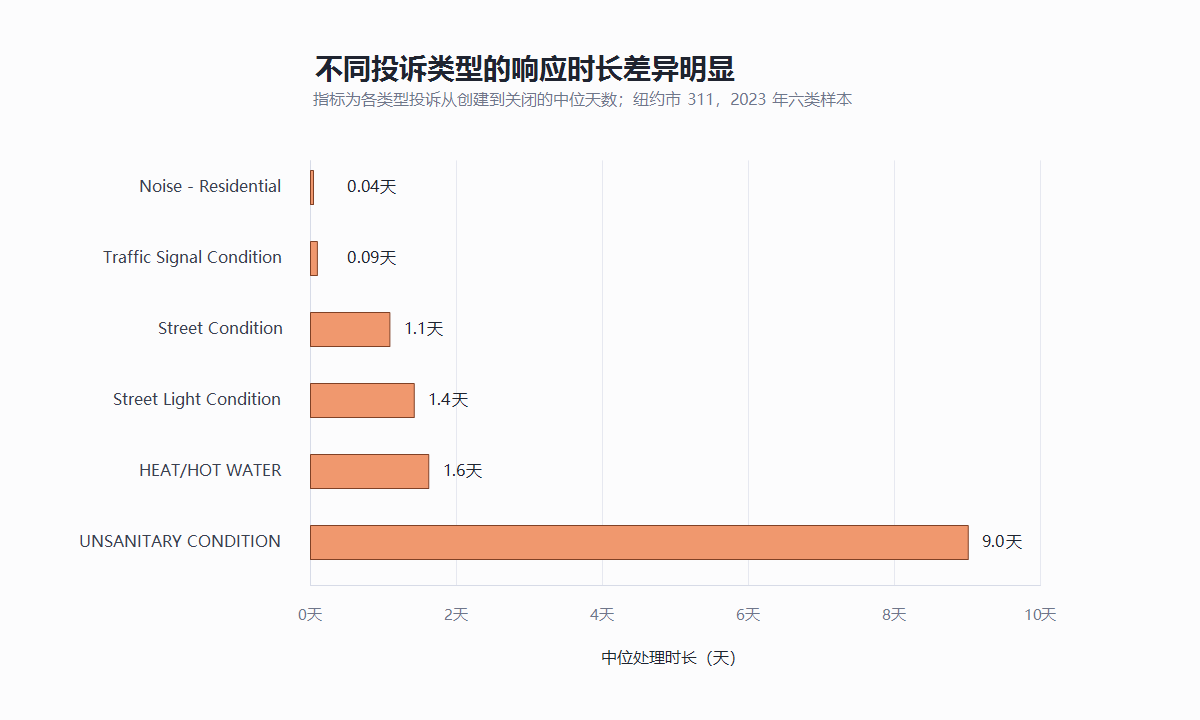
\includegraphics[width=0.85\textwidth]{fig1_complaint_type_median_equal_ticks.png}
\caption{不同投诉类型的中位响应时间}
\end{figure}

\subsection{空间差异存在}

从原始中位数看，Staten Island 响应最快，为 0.85 天；Manhattan 为 0.88 天；Bronx 最慢，为 1.19 天。但在使用对数调整模型控制投诉类型和月份后，Queens 的调整后响应时间比平均水平慢约 7.00\%，Brooklyn 慢约 6.29\%；Manhattan 快约 10.42\%，Staten Island 快约 13.43\%；Bronx 接近平均水平。这说明 Bronx 的原始慢响应部分来自投诉类型构成，而 Queens 和 Brooklyn 的部分慢响应更难完全由类型和月份解释。社区板层面，Queens 10、Queens 03、Bronx 04 等地区在控制投诉类型后仍明显慢于城市基准。
\begin{figure}[H]
\centering
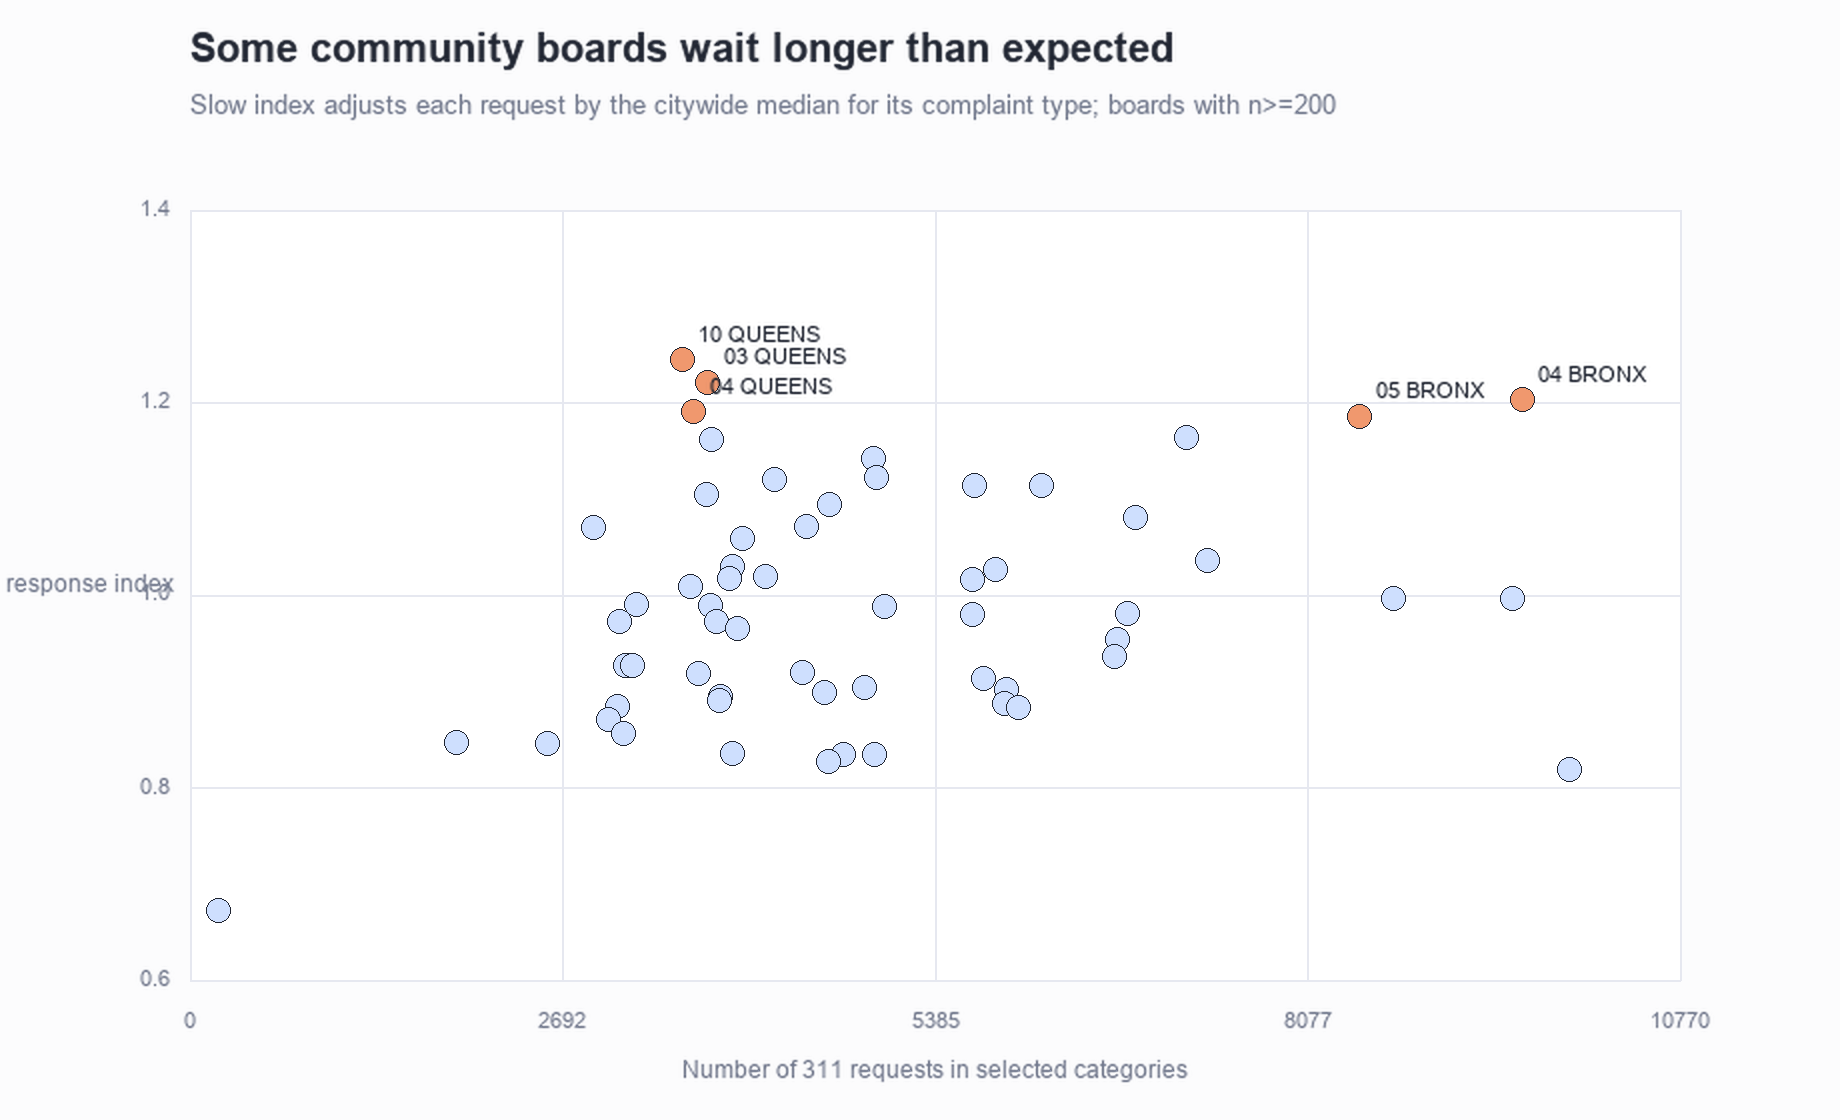
\includegraphics[width=0.85\textwidth]{figures/fig5_community_slow_index.png}
\caption{调整后的社区板慢响应指数 Top 10}
\end{figure}

\subsection{慢响应可以被提前识别}

基础模型中，投诉类型历史慢响应率基线 AUC 为 0.756，朴素贝叶斯为 0.760，基础 Logistic 为 0.796。目标编码 Logistic 在未来预测中 AUC 提升至 0.835，precision 和 recall 均为 0.606；在月份分层验证中 AUC 达到 0.919，precision 和 recall 均为 0.755。



\begin{table}[H]
\centering
\scriptsize
\caption{慢响应预测模型结果}
\label{tab:model_results}
\begin{tabular}{llccccc}
\toprule
验证方式 & 模型 & AUC & Precision & Recall & F1 & Accuracy\\
\midrule
未来预测 & 投诉类型基线 & 0.756 & 0.364 & 0.942 & 0.525 & 0.575\\
未来预测 & 朴素贝叶斯 & 0.760 & 0.481 & 0.482 & 0.482 & 0.741\\
未来预测 & 基础 Logistic & 0.796 & 0.524 & 0.524 & 0.524 & 0.762\\
未来预测 & 目标编码 Logistic & 0.835 & 0.606 & 0.606 & 0.606 & 0.803\\
月份分层 & 基础 Logistic & 0.904 & 0.729 & 0.729 & 0.729 & 0.864\\
月份分层 & 目标编码 Logistic & 0.919 & 0.755 & 0.755 & 0.755 & 0.878\\

\bottomrule
\end{tabular}
\end{table}

本文对比了不同预警比例的效果如表所示。目标编码 Logistic 在月份分层验证中显示，前 10\% 队列 precision 为 0.864 但 recall 仅 0.346；前 40\% 队列 recall 达到 0.895 但 precision 降至 0.559；前 25\% 队列 precision 和 recall 均为 0.755，F1 最高。因此，本文将预警比例设定为25\% 。


\begin{table}[H]
\centering
\scriptsize
\caption{不同预警比例下目标编码 Logistic 的识别效果}
\label{tab:alert_share}
\begin{tabular}{lrrrr}
\toprule
预警比例 & Precision & Recall & F1 & Accuracy\\
\midrule
前 10\% & 0.864 & 0.346 & 0.494 & 0.823\\
前 15\% & 0.830 & 0.498 & 0.623 & 0.849\\
前 20\% & 0.803 & 0.642 & 0.714 & 0.871\\
前 25\% & 0.756 & 0.756 & 0.756 & 0.878\\
前 30\% & 0.691 & 0.829 & 0.753 & 0.864\\
前 40\% & 0.559 & 0.895 & 0.689 & 0.798\\
前 50\% & 0.470 & 0.941 & 0.627 & 0.721\\
\bottomrule
\end{tabular}
\end{table}

重要特征也具有解释意义。UNSANITARY CONDITION 是强正向特征，说明卫生状况投诉最容易成为慢响应；Noise - Residential 和 Traffic Signal Condition 系数为负，说明住宅噪音和交通信号投诉更不容易进入最慢 25\%。

\begin{figure}[H]
\centering
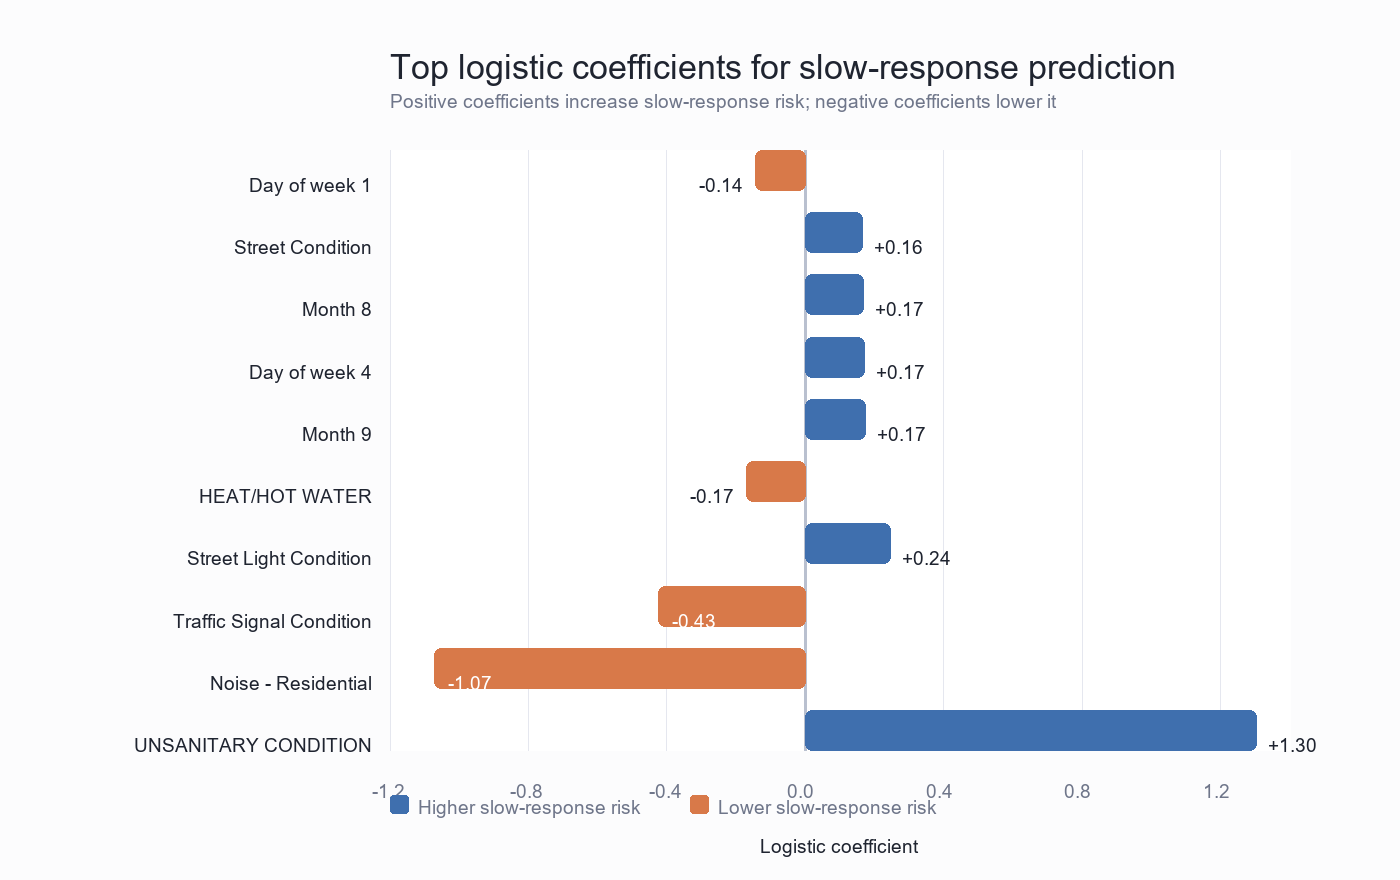
\includegraphics[width=0.85\textwidth]{fig8_top_features_fixed.png}
\caption{机制变量与慢响应率相关性}
\end{figure}

\subsection{机制变量解释区域聚集，而非替代个体预测}

加入 ACS、HPD 和工作量变量后，基础 Logistic 模型 AUC 从 0.79598 仅提高到 0.79608，提升极小。因此不能简单地说“低收入社区的每一条投诉都更慢”。

但在 ZIP 层面，机制变量具有明显解释价值。慢响应率与家庭收入中位数的相关系数为 -0.463（\(p<0.001\)）；与贫困率、HPD 住房违规数量和机构工作量的相关系数分别为 0.347（\(p<0.001\)）、0.353（\(p<0.001\)）和 0.202（\(p=0.008\)）。
\begin{figure}[H]
\centering
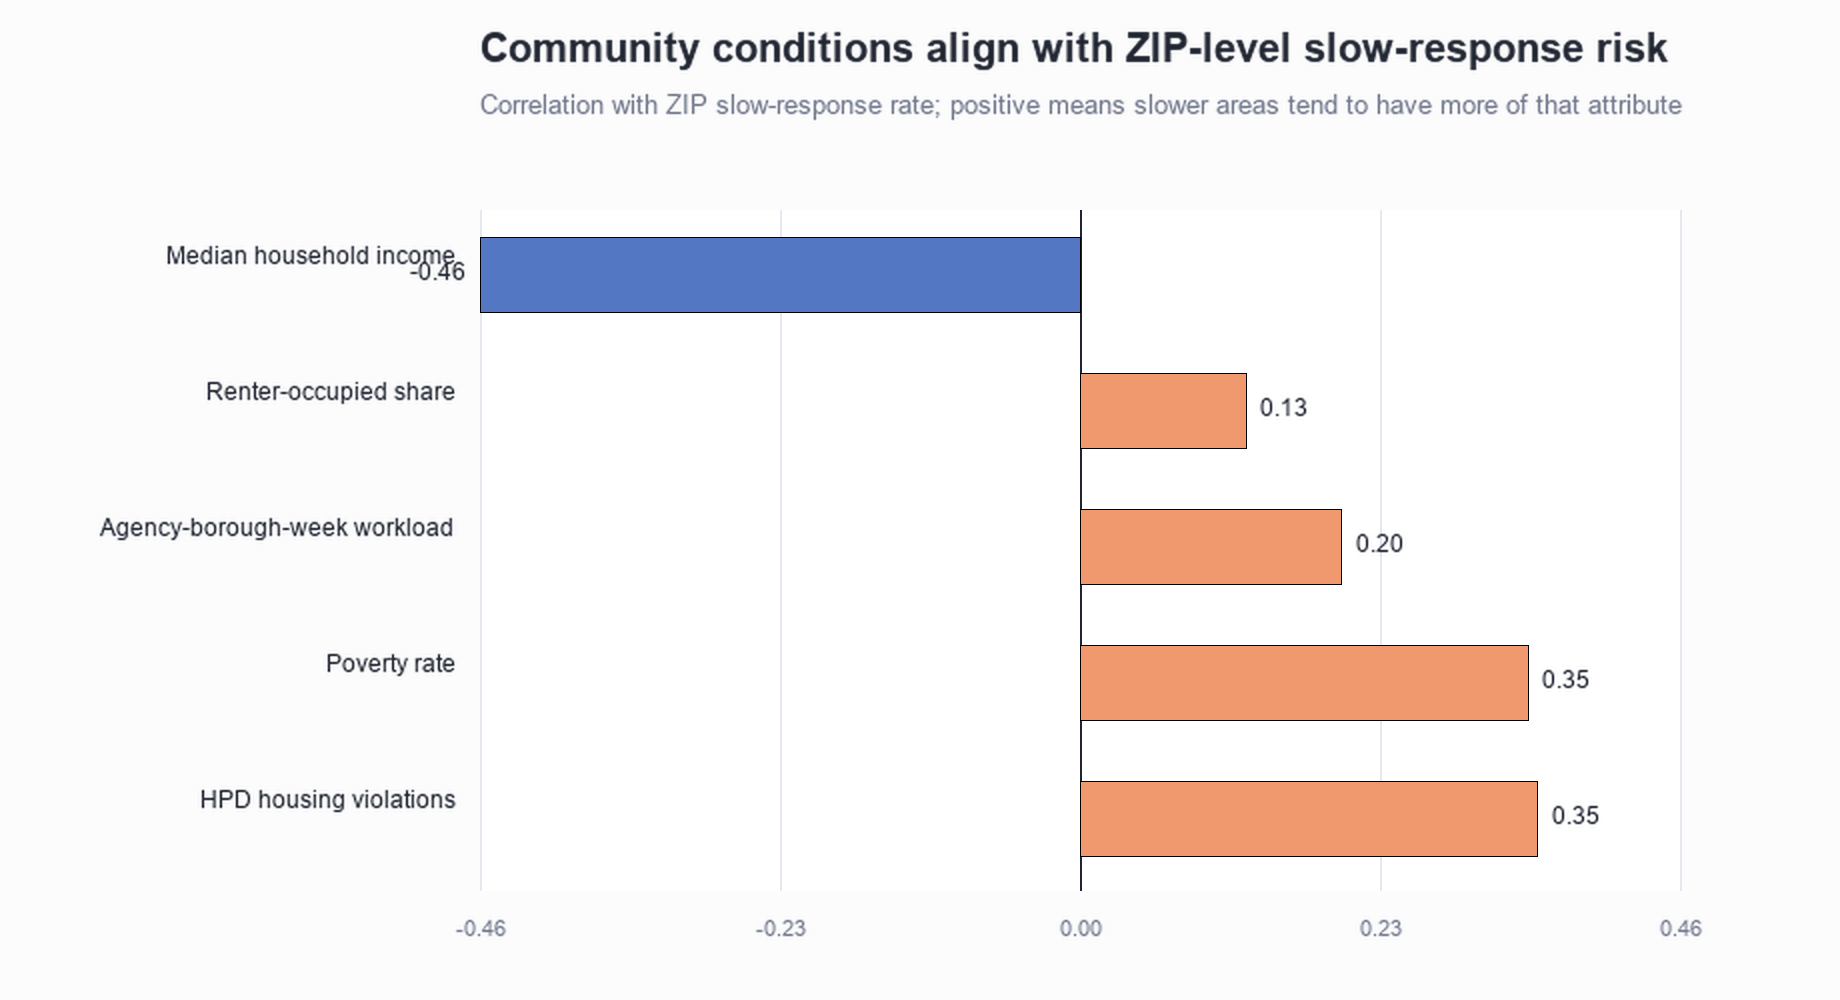
\includegraphics[width=0.85\textwidth]{figures/fig11_mechanism_correlations.png}
\caption{ZIP 层面机制变量与慢响应率相关性}
\end{figure}

异质性和面板结果见表 \ref{tab:hetero_panel}。低收入 ZIP 在交通信号投诉上的慢响应率高约 1.92 个百分点（\(p<0.001\)），但在路灯和卫生状况投诉上并不显著更慢；高住房违规 ZIP 在路灯投诉上的慢响应率高约 4.51 个百分点（\(p<0.001\)），在交通信号投诉上高约 1.65 个百分点（\(p<0.001\)）。面板固定效应结果显示，在控制 ZIP、月份和投诉类型后，工作量每上升 1 个标准差，慢响应率约提高 0.84 个百分点（\(p=0.044\)）。其置信区间下界接近 0，说明影响相对较弱。

\begin{table}[H]
\centering
\scriptsize
\caption{异质性分析与面板固定效应结果}
\label{tab:hetero_panel}
\begin{tabular}{llrrrr}
\toprule
检验 & 对象 & 效应(pp) & 标准误(pp) & 95\% CI(pp) & p值\\
\midrule
低收入ZIP & 供暖/热水 & -3.73 & 0.22 & [-4.16,-3.31] & <0.001\\
低收入ZIP & 路灯 & -0.59 & 0.84 & [-2.23,1.05] & 0.480\\
低收入ZIP & 交通信号 & 1.92 & 0.35 & [1.24,2.60] & <0.001\\
低收入ZIP & 卫生状况 & 0.07 & 0.36 & [-0.63,0.77] & 0.841\\
高HPD违规ZIP & 路灯 & 4.51 & 0.89 & [2.76,6.25] & <0.001\\
高HPD违规ZIP & 交通信号 & 1.65 & 0.36 & [0.94,2.36] & <0.001\\
高HPD违规ZIP & 卫生状况 & -1.03 & 0.36 & [-1.73,-0.34] & 0.004\\
面板固定效应 & 工作量1个标准差 & 0.84 & 0.42 & [0.02,1.66] & 0.044\\
\bottomrule
\end{tabular}
\end{table}

\subsection{时间序列、调度模拟与优化}

周度响应时间预测显示，4 周移动平均模型的平均绝对误差最低，为 0.180 天；最后观测值模型为 0.181 天；AR(1) 模型误差较高，为 0.815 天。这说明 311 响应时间具有短期惯性，简单移动平均已经可以用于监测未来几周服务压力。

为控制规模，本文从测试集中进行分层抽样，得到 1201 条投诉作为优化候选集。同时设定机构容量、投诉类型上限和行政区最低覆盖约束。

表 \ref{tab:ip_results} 显示，随机可行基准可节约 278.8 个等待天，捕捉 26.9\% 的慢响应案件。历史延迟 IP 将节约等待天数提高到 387.1，风险效率 IP 进一步提高到 464.0，并捕捉 51.8\% 的慢响应案件，是总等待时间节约最高的策略。公平加权 IP 的节约等待天数为 424.2，低于风险效率 IP，但其脆弱社区慢响应捕捉率达到 57.9\%，明显高于历史延迟 IP 和风险效率 IP 的 22.4\%。这说明，在多重资源约束下，风险效率策略最有利于降低总体等待时间，而公平加权策略可以用一定效率损失换取更高的脆弱社区覆盖。从效率角度看，风险效率 IP 是最优策略；从公平角度看，公平加权 IP 更符合公共服务均衡覆盖目标。二者的差异说明，优化模型不仅可以回答“优先处理哪些投诉最节约时间”，还可以回答“在节约时间和照顾脆弱社区之间如何权衡”。

\begin{table}[H]
\centering
\scriptsize
\caption{整数规划优化实验结果}
\label{tab:ip_results}
\begin{tabular}{lrrrrrr}
\toprule
策略 & 选中数 & 节约等待天 & 捕捉慢响应(\%) & 选中慢响应率 & 平均脆弱性 & 脆弱社区慢响应捕捉(\%)\\
\midrule
随机可行基准 & 296 & 278.8 & 26.9 & 0.274 & 0.534 & 34.2\\
历史延迟 IP & 280 & 387.1 & 43.5 & 0.468 & 0.440 & 22.4\\
风险效率 IP & 285 & 464.0 & 51.8 & 0.547 & 0.425 & 22.4\\
公平加权 IP & 272 & 424.2 & 48.8 & 0.540 & 0.566 & 57.9\\
\bottomrule
\end{tabular}
\end{table}

\section{讨论}

本文的政策含义可以分为三层。第一，绩效公开应按问题类型分开报告，不能只公布总体平均响应时间。第二，政府应定期计算慢响应指数，识别同类问题中持续慢于城市基准的社区。第三，高风险投诉预警应与资源调度结合：若目标是效率，应优先处理模型风险最高或预期收益最高的投诉；若目标是公平，应在优化模型中加入脆弱社区最低覆盖约束。对居民而言，若投诉属于卫生状况、住房维护、道路或路灯等复杂事项，且所在地区住房违规较多或部门负荷较高，等待时间更可能较长；此时持续追踪、保存编号并及时补充证据更重要。

本文也存在局限。第一，311 数据反映的是“被报告的问题”，不是所有真实问题；不同社区的报告意愿、数字能力和对政府的信任可能不同。第二，关闭时间不一定等于问题真正解决时间。第三，ZIP/ZCTA 匹配是近似空间匹配，ACS 和 HPD 变量也只是机制代理指标，能够说明相关性，但不能直接证明因果效应。未来研究可加入部门人员与预算、重复投诉和居民追踪记录。

\section{结论}

本文基于纽约 311 数据分析数字政务平台中的公共服务响应公平性。研究发现，响应差异首先来自投诉类型，其次体现为空间不均衡；慢响应可以被提前预测，且区域慢响应与收入、贫困、住房违规和部门负荷有关。优化实验进一步说明，预测模型只有转化为资源分配规则才具有政策意义：风险优先更有利于降低总等待时间，公平约束最优解更有利于覆盖脆弱社区。本文t通过构建慢响应指数、机制变量、预测模型、时间序列监测和调度优化共同构成了一套可解释的数据挖掘框架，可帮助城市管理者识别服务响应中的薄弱环节，并为更公平的公共服务配置提供依据。

\begin{thebibliography}{9}
\bibitem{wang2016} Wang, L., Qian, C., Kontokosta, C., \& Sobolevsky, S. (2016). Structure of 311 Service Requests as a Signature of Urban Location.
\bibitem{kontokosta2017} Kontokosta, C., Hong, B., \& Korsberg, K. (2017). Equity in 311 Reporting: Understanding Socio-Spatial Differentials in the Propensity to Complain.
\end{thebibliography}

\end{document}
